\documentclass[compress,handout,10pt]{beamer}

\newlength{\wideitemsep}
\setlength{\wideitemsep}{\itemsep}
\addtolength{\wideitemsep}{100pt}
\let\olditem\item
\renewcommand{\item}{\setlength{\itemsep}{0.5\baselineskip}\olditem}

\usetheme{Singapore}
\usecolortheme{lily}
\usefonttheme[onlymath]{serif}

\usepackage{float}
\floatstyle{boxed}
\usepackage{colortbl}
\usepackage{mathpazo}
\usepackage{graphicx}
\usepackage{movie15}
\usepackage{bm}
\usepackage{verbatim}
\usepackage{comment}
\usepackage{caption}
\usepackage{subcaption}
\captionsetup[subfigure]{labelformat=empty}
\captionsetup[figure]{labelformat=empty}

\newcommand{\mygreen}{\color{green!50!black}}
\newcommand{\myblue}{\color{blue}}
\newcommand{\myred}{\color{red}}
\newcommand{\mycolor}{\color{red}{c}\color{blue}{o}\color{green}{l}\color{orange}{o}\color{cyan}{r}}
\newcommand{\mysize}{\scriptsize{s}\small{i}\normalsize{z}\Large{e}}
\newcommand{\myshape}{\textcircled{s}\textit{h}\texttt{a}\textsf{p}\textsc{e}}

\xdefinecolor{titlecolor}{rgb}{.855,.647,.125}
\setbeamercolor{frametitle}{fg=titlecolor}
\setbeamerfont{frametitle}{series=\bfseries}
\setbeamercolor{normal text in math text}{parent=math text}

\setbeamertemplate{navigation symbols}{} %gets rid of navigation symbols
\setbeamertemplate{footline}[frame number]
\beamertemplateshadingbackground{blue!5}{yellow!10}

\title{{\color{blue} \LARGE Dungeness Crab Growth\newline} }

\subtitle{{\color{red} \large National Marine Fisheries Service} }

\author{ 
%    \vspace{5pt}
    {Xiaohan Yang} \\ 
    \vspace{5pt}
} 
\institute{Johns Hopkins University}

\date{\mygreen \today} 

\begin{document}

\begin{frame}[plain]
    \titlepage
\end{frame}

\begin{frame}
    \frametitle{Outline}
    \tableofcontents
\end{frame}

\section{Background}

\begin{frame}
    \frametitle{Introduction to National Marine Fisheries Service}
    \vspace{7pt}
             \begin{enumerate}
                 \item Federal agency and a division of the Department of Commerce
                 \item Manage, conserve and protect living marine resources and their habitats
                 \item Promote sustainable fisheries and prevent overfishing
                 \item Balance competing public needs
             \end{enumerate}
\end{frame}

\section{Problem Statement}
\begin{frame}
    \frametitle{Problem Raised by the Fishing of Dungeness Crabs}
     \begin{enumerate}
         \item A species living along the Pacific coast of North America
         \item Male crabs are fished during December and June. Female crabs are not fished. It leads to a large ratio of female to male crabs.
         \item Great fluctuations in the catches of crabs
         \item Decrease in crab population along the central California coast
         \item Female Dungeness crabs are considered to be fished.
     \end{enumerate}
\end{frame}

\begin{frame}
    \frametitle{My Project}
     \begin{enumerate}
         \item Size restrictions on female crabs have to be set so that crabs can mate at least once before they are caught.
         \item Growth of crabs needs to be studied so that scientists can set the size of the fishing net to meet the restriction.
         \item Crabs mate during the molting season of female crabs. So I need to study the change of sizes by molting.
         \item Predict the premolt size from the postmolt size
     \end{enumerate}
\end{frame}

\section{Deliverable}

\begin{frame}
    \frametitle{From Team to Sponsor}
    The following outputs are expected from this project:
     \begin{enumerate}
         \item A regression formula predicting premolt sizes from postmolt sizes of female Dungeness crabs taken the place of molting into consideration
         \item A R programming package which can predict the premolt sizes of shells and produce a graph for the distribution of premolt sizes when people input the data of postmolt sizes of shells and the place of molting in the program
     \end{enumerate}
\end{frame}

\begin{frame}
    \frametitle{From Sponsor to Team}
    In order for my project to be of successful one, I will need:
     \begin{enumerate}
         \item Data of shell sizes before molting and corresponding postmolt sizes specifying the molting environment and measurement year. The data should be delivered to me by Oct 12, 2012. If my sponsor fails to do so, I will only develop a method for the prediction problem without an explicit regression formula.
         \item Computing resources
         \item Timely responses to inquiries, 
         \item Symposium attendance travel expenses.
     \end{enumerate}
\end{frame}

\section{Approach}
\begin{frame}
    \frametitle{Collection of Data}
    The data were collected in the following ways:
     \begin{enumerate}
         \item Place: northern California and southern Oregon
         \item Time: Year 1981, 1982 and 1992
         \item Type of data: laboratory data and capture-recapture data
     \end{enumerate}
\end{frame}

\begin{frame}
    \frametitle{Selecting Data}
    I need to do the following things to the data to make them suitable for my project:
     \begin{enumerate}
         \item Secondary data
         \item Delete data without premolt size or postmolt size or data type
         \item Delete outliers
         \item 472 data left with $\frac{3}{4}$ of them laboratory data
     \end{enumerate}
\end{frame}

\begin{frame}
    \frametitle{Data}
    After adjustments, part of the data are shown in the following table:
    \begin{figure}
        \begin{center}
	    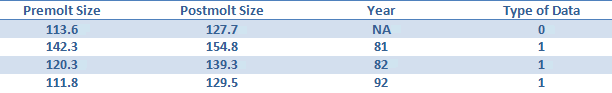
\includegraphics[width=\textwidth]{data.png}
	\end{center}
	\caption{Part of Data after Adjustments}
    \end{figure}
\end{frame}

\begin{frame}
    \frametitle{Methods}
     \begin{enumerate}
         \item Software: R
         \item Linear regression model with postmolt size and data type as independent variables and premolt size as dependent variable
         \item Ordinary least squres method to find the coefficient
         \item Analysis of Variance to test the significance level of the coefficient and the performance of the model
         \item Refine the model
     \end{enumerate}
\end{frame}

\begin{frame}
    \frametitle{Form of the Model}
     My model in the very beginning is in the following form:
     $$Premolt~Size=\beta_0 + \beta_1 (Postmolt~Size) + \beta_2 (Type~of~Data)$$
     One way to refine:
     \begin{align*}
      Premolt~Size = ~&\beta_0 + \beta_1 (Postmolt~Size) + \beta_2 (Type~of~Data)\\
               & + \beta_3 (Postmolt~Size)*(Type~of~Data)
     \end{align*}
     Another way to refine:
     \begin{align*}
      Premolt~Size = ~&\beta_0 + \beta_1 (Postmolt~Size) + \beta_1 (Postmolt~Size)^2\\
               & + \beta_3 (Type~of~Data).
     \end{align*}
\end{frame}

\section{Conclusion}
\begin{frame}
    \frametitle{Work Remaining to Be Done}
     \begin{enumerate}
         \item Find the coefficients for the simplest linear model
         \item Test the model
         \item Refine the model
     \end{enumerate}
\end{frame}

\begin{frame}
    \frametitle{Recommendations for Future Research}
     \begin{enumerate}
         \item Take the time into consideration
         \item Take the types of crab shells into consideration
     \end{enumerate}
\end{frame}

\begin{frame}[allowframebreaks]{Bibliography}
    \frametitle{References}
        \bibliographystyle{plain}
        \nocite{*}
        \bibliography{biblio}
\end{frame}

\end{document}
